\section{Experimental Protocol}
\label{sec:experimental_protocol}

The experimental protocol is designed to evaluate both in-domain performance and cross-dataset generalization while preventing test leakage. All models are trained on a single source domain, LOL-v2 Real, and the validation split is used for early stopping, checkpoint selection, and model selection. The test sets are never used during these steps and are evaluated only after the final configuration has been selected.

The project is organized around model families. For each family, a dedicated grid search explores meaningful architectural and optimization choices, while the other parts of the experimental procedure are kept unchanged whenever possible. These common parts include the data augmentation policy, the training and validation procedure, and the validation-based selection strategy. In this way, different model families can be compared under consistent experimental conditions and under a similar computational budget.

Across comparable runs, the training setup keeps fixed the batch size, the data-loading strategy, the validation frequency, the use of mixed precision when supported by the hardware, and the choice of favoring efficiency over fully deterministic execution. The maximum number of training epochs is intentionally set as a large upper bound, because the effective training duration is controlled by early stopping rather than by a fixed epoch budget.

Early stopping is implemented in a model-agnostic way. The monitored validation metric, its optimization direction, and the optional tie-breaker metric can be selected according to the specific experiment or model family. However, the overall early-stopping policy is kept fixed across comparable runs, so that all configurations are selected according to the same validation-based logic.

For each model family, the experimental protocol is organized into the following stages: (i) a screening stage, in which all configurations of the grid search are trained with a fixed seed and ranked using validation performance; (ii) a multi-seed re-training stage, in which the most promising configurations are re-trained with multiple random seeds to estimate both performance and stability; (iii) a validation-based model selection stage, in which the final configuration is chosen from the aggregated multi-seed validation results; and (iv) a final evaluation stage, in which the selected configuration is tested on the in-domain test set and on all cross-dataset test sets. During screening and model selection, test evaluation is disabled; it is enabled only in the final evaluation stage. Figure~\ref{fig:experimental_protocol} provides a visual overview of this workflow, while the following subsections describe each stage in detail.

\begin{figure*}[t]
    \centering
    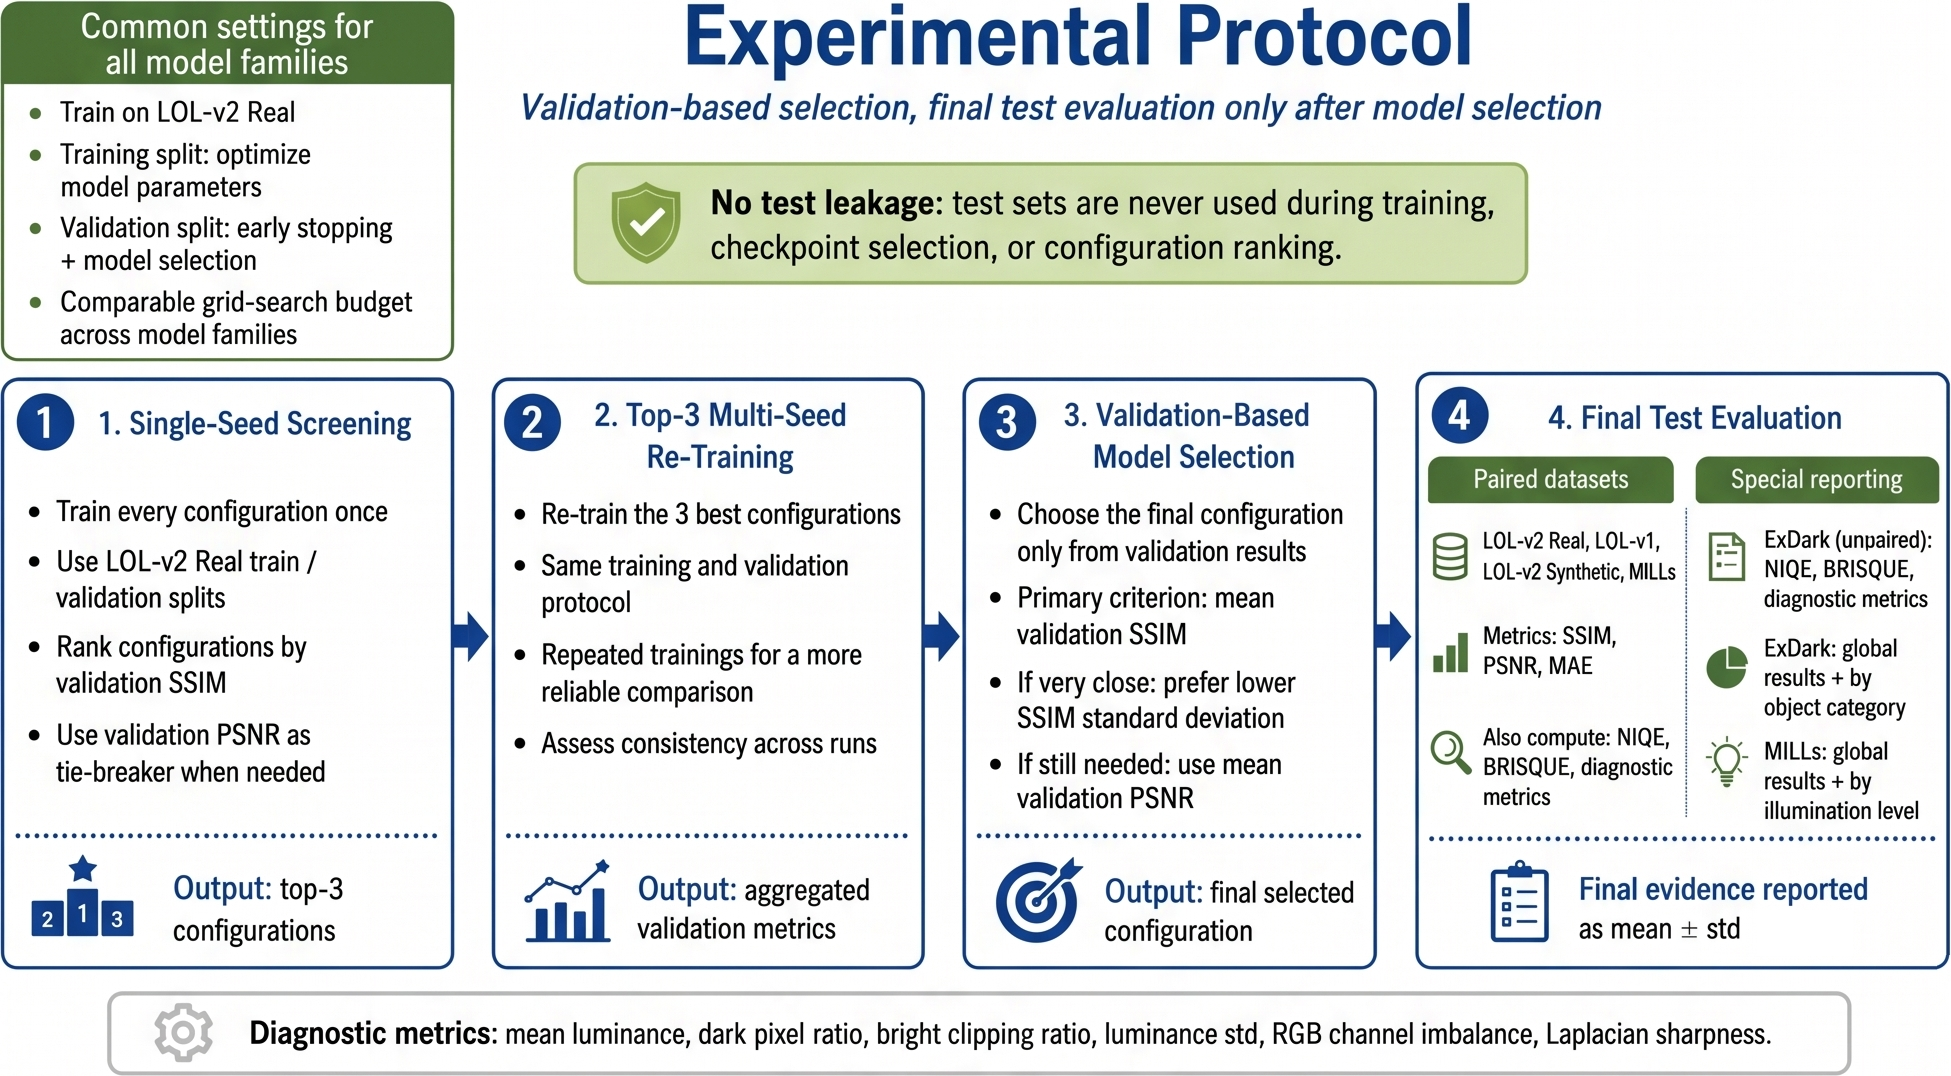
\includegraphics[width=\textwidth]{fig/experimental_protocol/experimental_protocol.png}
    \caption{Overview of the experimental protocol.}
    \label{fig:experimental_protocol}
\end{figure*}

\subsection{Single-Seed Screening}

The first experimental stage is a single-seed grid search, in which every configuration is trained using a single fixed seed. The purpose of this stage is not to produce final evidence, because a single seed can be affected by random initialization and data-loader randomness. Instead, the purpose is to reduce the search space and identify a small number of promising configurations.

Each configuration is trained on the LOL-v2 Real training split and monitored on the LOL-v2 Real validation split. The test sets are not evaluated during screening. For each run, validation structural similarity index measure (SSIM)~\cite{DBLP:journals/tip/WangBSS04} is used as the primary criterion for checkpoint selection. This choice reflects the goal of low-light enhancement: the output should remain structurally similar to the reference image, preserving luminance, contrast, and local image structure, rather than only reduce the average pixel-wise error. Validation peak signal-to-noise ratio (PSNR) is also computed and used as a tie-breaker because it measures pixel-wise reconstruction quality in logarithmic form. Therefore, when two checkpoints achieve validation SSIM values within the configured tolerance, PSNR is used to select the best checkpoint for that run.

The output of this stage is a validation-based ranking of the explored configurations. This ranking is later parsed from the run logs and used to select the top-3 configurations for the multi-seed stage.

\subsection{Top-3 Multi-Seed Re-Training}

After the screening stage, the three most promising configurations are selected from the validation-based ranking and re-trained under the same training and validation protocol. This stage is necessary because the screening phase provides only a preliminary estimate of performance, obtained from a single training run for each configuration.

The goal of the multi-seed stage is to obtain a more reliable comparison among the selected configurations. By repeating the training procedure several times for each of them, the protocol can evaluate whether its validation performance is consistent or mainly due to a favorable run.

The outputs of this stage are aggregated validation metrics for each selected configuration. These aggregated results are then used for the final validation-based selection, while the test sets remain untouched.

\subsection{Validation-Based Model Selection}

The final configuration is selected only from the aggregated validation results of the multi-seed stage.

The primary selection criterion is the mean validation SSIM across runs. When configurations obtain very close mean SSIM values, the selection favors the more stable configuration, measured by the standard deviation of validation SSIM. If the comparison is still ambiguous, mean validation PSNR is used as a final tie-breaker.

This rule keeps the whole selection process validation-based, while also accounting for statistical robustness across repeated trainings.

\subsection{Final Test Evaluation}

The final test evaluation is performed only after the final configuration has been selected. The selected configuration is evaluated on the test set of all the datasets used in this project, and the resulting metrics are aggregated as mean and standard deviation. This ensures that the final evidence is not based on a single run, but reflects both average performance and statistical robustness.

The evaluation protocol depends on whether a dataset is paired or unpaired. In paired datasets, ``full-reference'' metrics can be computed by comparing the enhanced output of the model with the corresponding target image of the dataset. In this work, paired datasets are evaluated using SSIM, PSNR, and mean absolute error (MAE). This last metric measures the average absolute pixel difference between the enhanced image and the reference image.

``No-reference'' metrics do not require target images and are computed for both paired and unpaired datasets. In this work, the no-reference metrics are naturalness image quality evaluator (NIQE)~\cite{DBLP:journals/spl/MittalSB13} and blind/referenceless image spatial quality evaluator (BRISQUE)~\cite{DBLP:journals/tip/MittalMB12}. More specifically, NIQE measures the deviation of an image from statistical properties commonly observed in natural images, while BRISQUE estimates perceptual quality from spatial scene statistics.

Additional diagnostic metrics are computed on the model output for both paired and unpaired datasets. They are used to support the interpretation of failure modes, meaning recurring types of enhancement errors. These diagnostics include: (i) mean luminance, which measures the average brightness of the enhanced image; (ii) dark pixel ratio, which measures the fraction of pixels that remain very dark; (iii) bright clipping ratio, which measures the fraction of pixels close to saturation; (iv) luminance standard deviation, which provides a compact indication of contrast variation; (v) red-green-blue (RGB) channel imbalance, which helps detect color cast; and (vi) Laplacian sharpness, which provides a simple estimate of high-frequency content related to blur, noise, or halo artifacts.

LOL-v1 and LOL-v2 are paired datasets and are therefore evaluated by aggregating full-reference metrics, no-reference metrics, and diagnostic output metrics over their respective test sets. ExDark and MILLs require a more specialized reporting protocol because of their particular dataset structure and evaluation objectives.

For ExDark, which is unpaired, no normally exposed target image is available. Therefore, it is evaluated using only no-reference metrics and diagnostic output metrics. In addition to global results over the whole dataset, ExDark is also analyzed by object category, since its images are organized into semantic groups.

MILLs is a paired dataset and is therefore evaluated similarly to LOL-v1 and LOL-v2. However, its results are reported at two levels: globally across all samples and separately by illumination level. This grouped reporting is particularly useful because MILLs includes inputs captured under different illumination conditions, enabling a more detailed analysis of how model performance varies with illumination.